\section{Experiments}
\label{sec:experiments}

%Unlike regular crowdsourcing, there is no publicly available platform for running real-world spatial crowdsourcing campaigns. With platforms such as Amazon Mechanical Turk, workers do not perform spatial crowdsourcing tasks. For this reason, we simulated various spatial crowdsourcing campaigns on an Inter(R) Core(TM)2 Duo 3.16GHz PC with 4GB memory running Microsoft Windows 7.

\subsection{Dataset}
\label{subsec:dataset}
Due to its commercial value, real-life SC systems such as Uber and TaskRabbit do not make their datasets available to public. We evaluate our algorithms using real check-in data in Foursquare and Gowalla and convert them spatial tasks and workers in our system. We consider check-ins as a spatial task performed at the location the check-in happened. For each location, we consider all check-ins within a two hours duration. For each task, we set the release time and deadline to the first and last check-in time within the two hours duration. We consider each user as a spatial worker with start and end times equal to the user's first and last check-in during a day. We select the initial location of a worker as a random point within the bounding box of all checked-in locations of the corresponding user. We also measure the travel time with the Euclidean distance between two points divided by an average speed of $60 km/h$. We use the data from 5 metropolitan areas: New York, Los Angeles, Paris, London \& Beijing. 

\cref{tab:flickr_stats} shows the total number of tasks (and workers) for each city.

\begin{table}[h]
\begin{center}
\begin{tabular}{| l || c | c |} \hline
			&	\# of Tasks	&	\# of Workers	\\ \hline
Los Angeles	&	219,332		&		19,081		\\ \hline
New York	&	390,229		&		17,603		\\ \hline
London		& 	366,034		&		18,480		\\ \hline
Paris		&	237,344		&		14,275		\\ \hline
Beijing		&	23,335		&		1,598		\\ \hline
\end{tabular}
\vspace{-0.1in}
\caption{\small{Number of tasks/worker for each city in Flickr dataset}}
\label{tab:flickr_stats}
\end{center}
\end{table}

We also generated a synthetic dataset with realistic streaming workload using \cite{To15}. To generate a workload suitable for SC systems we modeled three different sets of parameters:
%We also generated a synthetic dataset with realistic streaming workload based on the methodology proposed in \cite{Tang07}. To generate a workload suitable for SC systems we modeled three different sets of parameters:

\noindent \textbf{Temporal Parameters:} In \cite{Basu15}, it is shown that with crowdsourcing environments, workers and tasks arrive following Poisson processes \cite{Stoyan87}.The default Poisson arrival rates for tasks and workers are \boldmath$\mu_t = 20/min$ and $\mu_w = 3/min$, respectively. Subsequently, the duration of the tasks and workers were randomly sampled from closed range of \boldmath{$\left[1,4 \right]$} \textbf{hours} and $\left[1,8 \right]$ \textbf{hours}, respectively.

\noindent \textbf{Spatial Parameters:} \cref{fig:la_gowalla} shows the spatial distribution of tasks from our real-world dataset in Los Angeles. As depicted, the tasks are not uniformly distributed in space. The spatial distribution is rather skewed, meaning that the density of the tasks at certain areas is higher. To model the same behavior with our synthetic workloads, we created 6 two dimensional Gaussian clusters with randomly selected means and standard deviations. Eighty percent of the tasks are sampled within the clusters and the rest are uniformly distributed.

\noindent \textbf{Static Parameters:} In addition to the spatiotemporal parameters, we consider two other parameters. The default \emph{workload size} of each experiment is \textbf{50K tasks}. The task arrival rate and the number of tasks determine the duration of the simulation. Based on the duration of the simulation and the worker arrival rate, the total number of workers may vary.\\
The maximum number of tasks a worker can perform, i.e., $w_{max}$, is a uniformly random number from the closed interval \boldmath$\left[8,12 \right]$.

\begin{figure}[h]
	\centering
	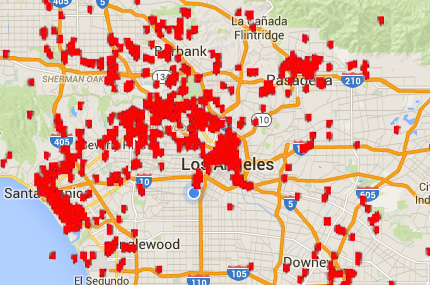
\includegraphics[scale=0.35]{figures/la_flickr.jpg}
	\caption{Spatial Distribution of Tasks in Gowalla}\label{fig:la_gowalla}
\end{figure}

%\subsection{Online vs. Offline}
%As the first set of experiments, we compare how the results of the real-time algorithms compare with the optimal solution computed using the offline clairvoyant algorithm explained in \cref{sec:exactalgo}. Because of the high complexity of the offline algorithm, we are not able to run tests with large workloads and thus we use workloads with 100 tasks. The experimental results of \cref{fig:off_vs_on} show that the best real-time algorithms perform close to \textasciitilde 60\% of the optimal solution. Our results are consistent with studies that compute a \emph{competitive ratio} \cite{Sleator85} of $1 - e^{-1}$ for the online matching problem with random inputs \cite{Goel08}.

%\begin{figure}[h]
%	\centering
%	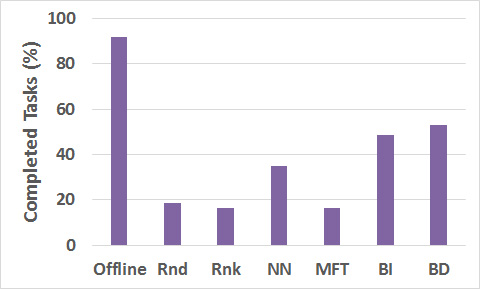
\includegraphics[width = 0.6\columnwidth]{figures/off_vs_on.jpg}
%	\caption{Comparison of Offline and Real-time approaches}\label{fig:off_vs_on}
%\end{figure}

\subsection{Experiment Setup}
\label{subsec:exp_setup}

In our experiments, we evaluate two different aspects of our framework. First, we compare the assignment quality of the proposed algorithms, i.e., the percentage of tasks the are completed. We compare the assignment quality of Auction-SC with the batched assignment framework (BATCHED) from \cite{Deng15}. We also compare the assignment quality of SC bidding rules with non-SC bidding rules (\cref{subsec:bidding}). Following, we evaluate the scalability of Auction-SC. In addition to comparing the scalability of Auction-SC with BATCHED, we also show that a monolithic server is not able to scale as high as Auction-SC.




\subsection{Assignment Quality}
In this section we evaluate the quality of the assignments using different real-time non-clairvoyant algorithms. First, we compare them using the Flickr and the synthetic datasets. Subsequently, using the synthetic datasets, we show how the spatial and temporal settings of the problem can affect the performance of the real-time assignment quality.

\begin{figure}[h]
    \centering
    \subfigure[Gowalla]{
        \label{fig:gowalla}
        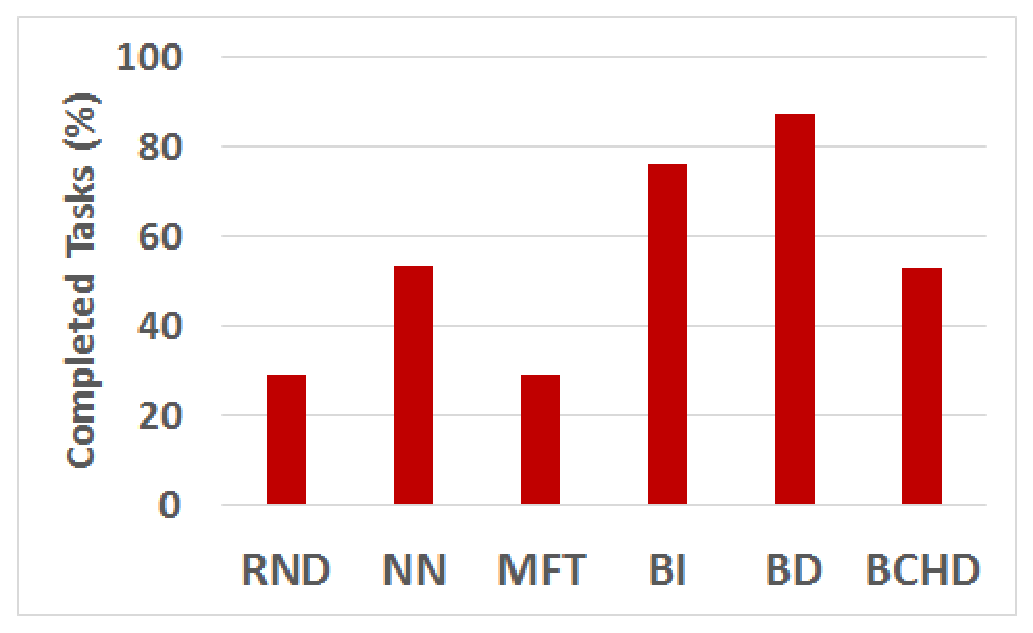
\includegraphics[width = 0.45\columnwidth]{figures/gowalla.eps}
    }
    \subfigure[Foursquare]{
        \label{fig:foursquare}
        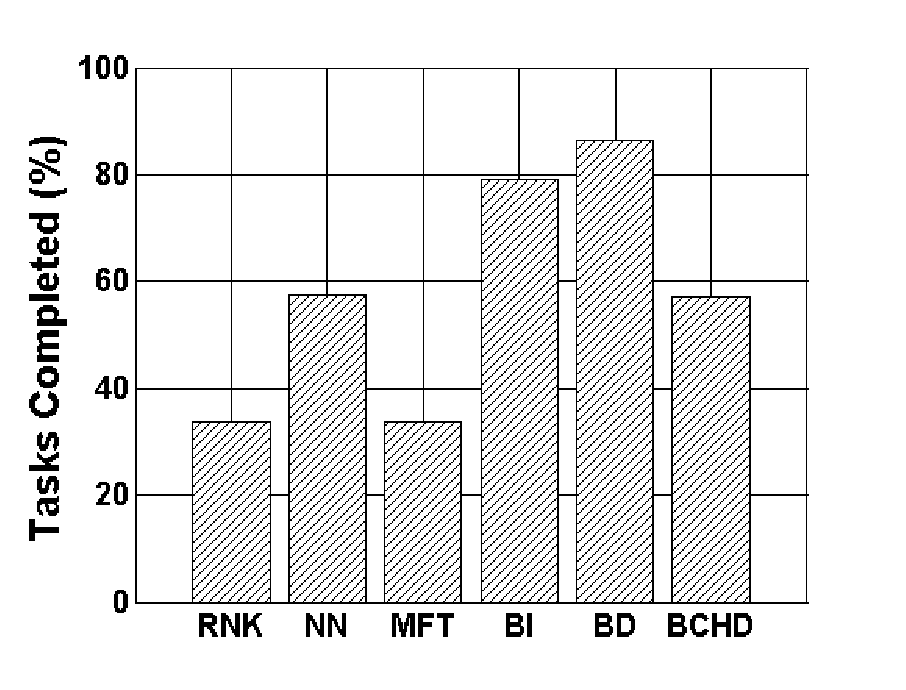
\includegraphics[width = 0.45\columnwidth]{figures/foursquare.eps}
    }
    \subfigure[Synthetic]{
        \label{fig:syn}
        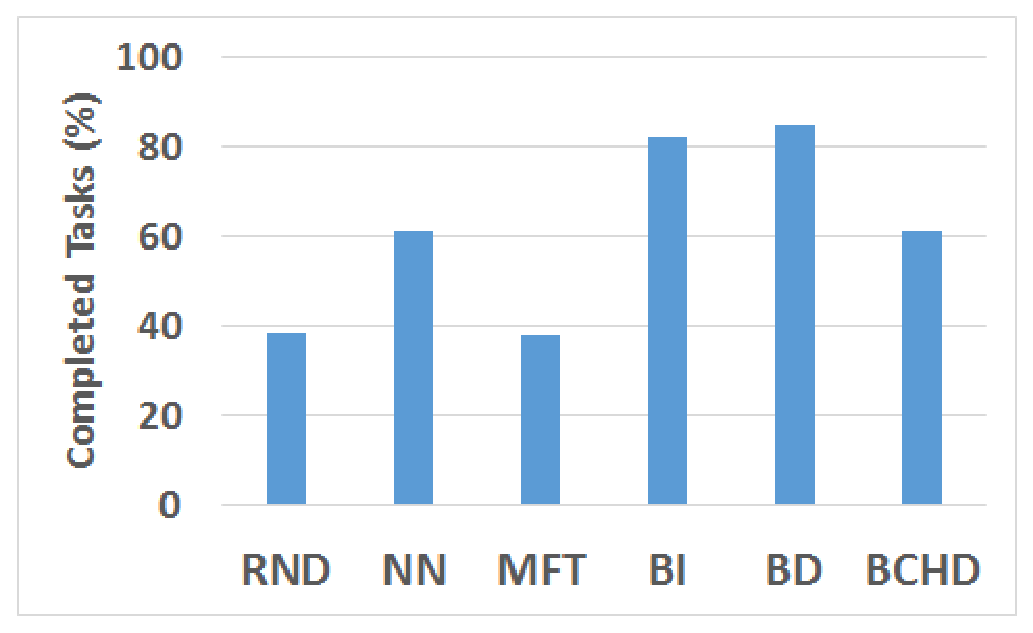
\includegraphics[width = 0.45\columnwidth]{figures/syn.eps}
    }
    \vspace{-0.15in}
    \caption{Assignment Quality of Real-Time Approaches}
    \label{fig:quality}
\end{figure}

\cref{fig:quality} compares the assignment quality of different real-time algorithms. As we can see, both SC approaches outperforms the best non-SC algorithm by almost 25\%. The main reason as explained in \cref{sec:onlinealgo} is that, the SC rules perform scheduling when matching tasks with workers. Furthermore, the BD approach outperforms BI by at most 10\%. This is not surprising as BD tends to ``move" workers to areas where future tasks are more likely to appear, thus achieving higher assignment in long term. Among the non-SC approaches NN outperforms other rules by almost 2 times more completed tasks. The reason MFT does not outperform baseline approaches (Rnd and Rnk) can be explained by what we call a \emph{radical move}. A \emph{radical move} is when the SC-Server assigns a task to a worker which requires it to move a relatively long distance to reach the location of that task. Since we do not consider any spatial proximity to the task with MFT, there is a high chance to end up with assignments resulting in radical moves. With NN and BI the general idea is to prevent radical moves as much as possible. With BD, although radical moves occur, but only if the worker moves to areas where there will be more tasks to complete. 

\begin{figure}[h]
    \centering
    \subfigure[RNK]{
        \label{fig:rnk_comp}
        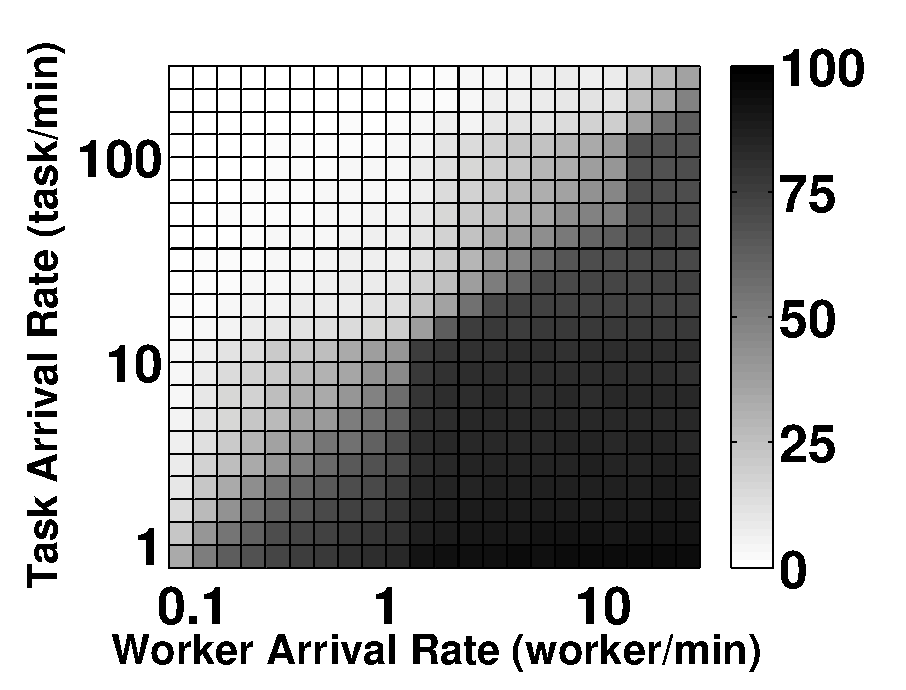
\includegraphics[width = 0.45\columnwidth]{figures/rnk.eps}
    }
    \subfigure[MFT]{
        \label{fig:mft_comp}
        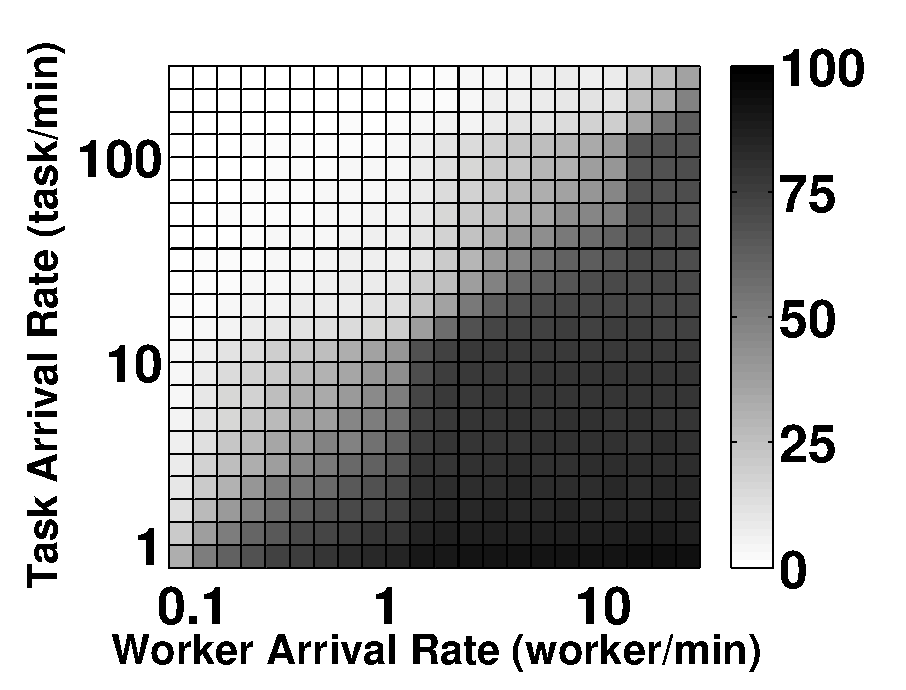
\includegraphics[width = 0.45\columnwidth]{figures/mft.eps}
    }
    \subfigure[NN]{
        \label{fig:nn_comp}
        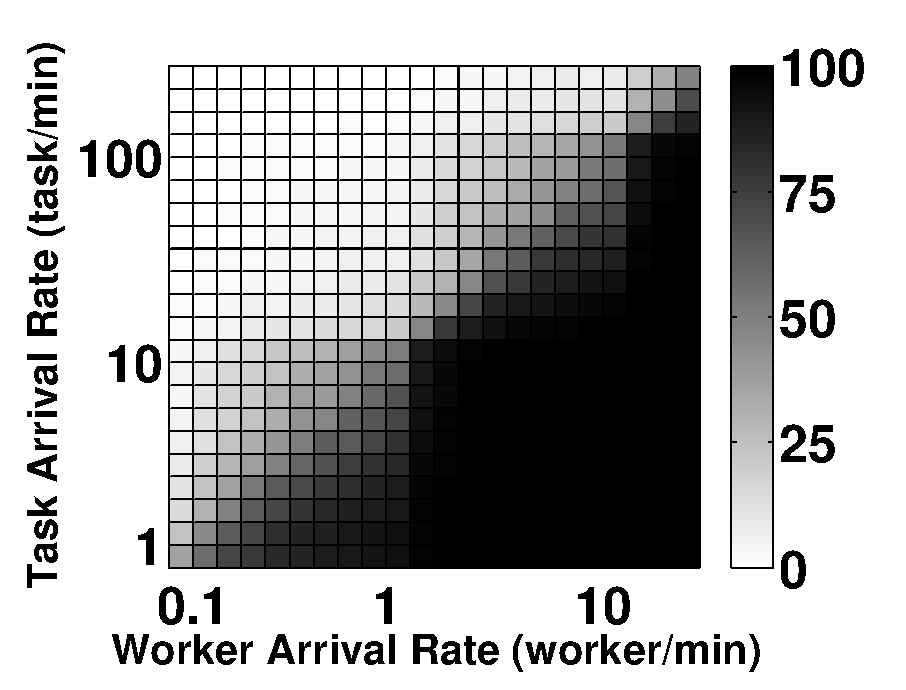
\includegraphics[width = 0.45\columnwidth]{figures/nn.eps}
    }
    \subfigure[BI]{
        \label{fig:bi_comp}
        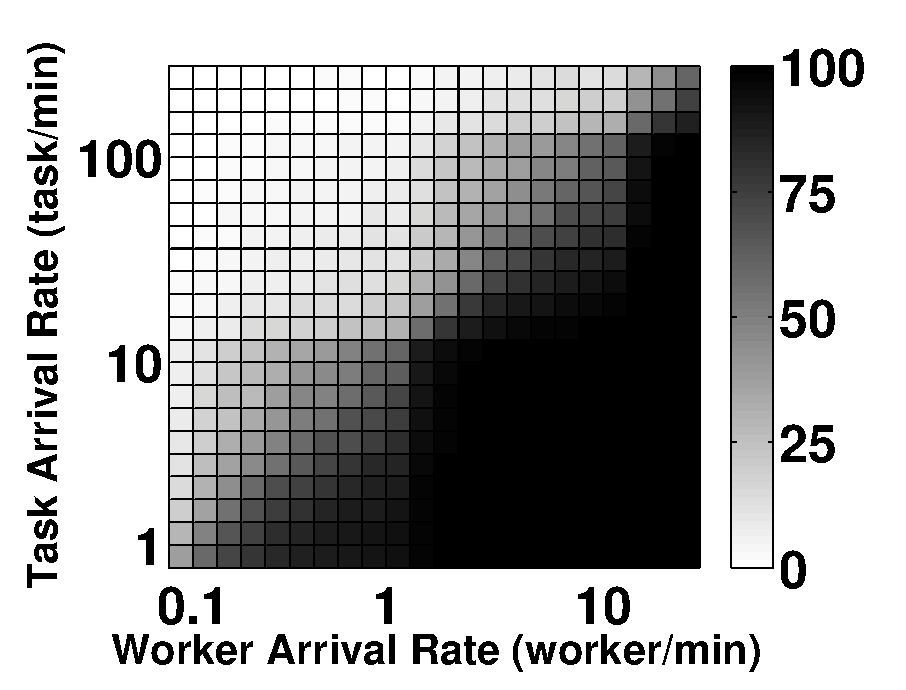
\includegraphics[width = 0.45\columnwidth]{figures/bi.eps}
    }
    \subfigure[BD]{
        \label{fig:emd_comp}
        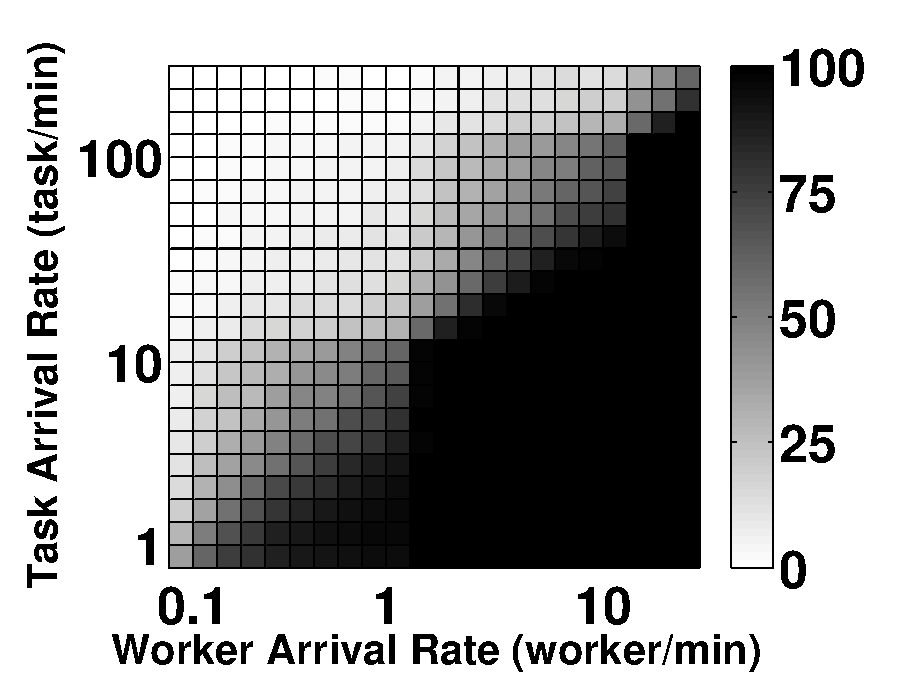
\includegraphics[width = 0.45\columnwidth]{figures/emd.eps}
    }
    \subfigure[BCHD]{
        \label{fig:bchd_comp}
        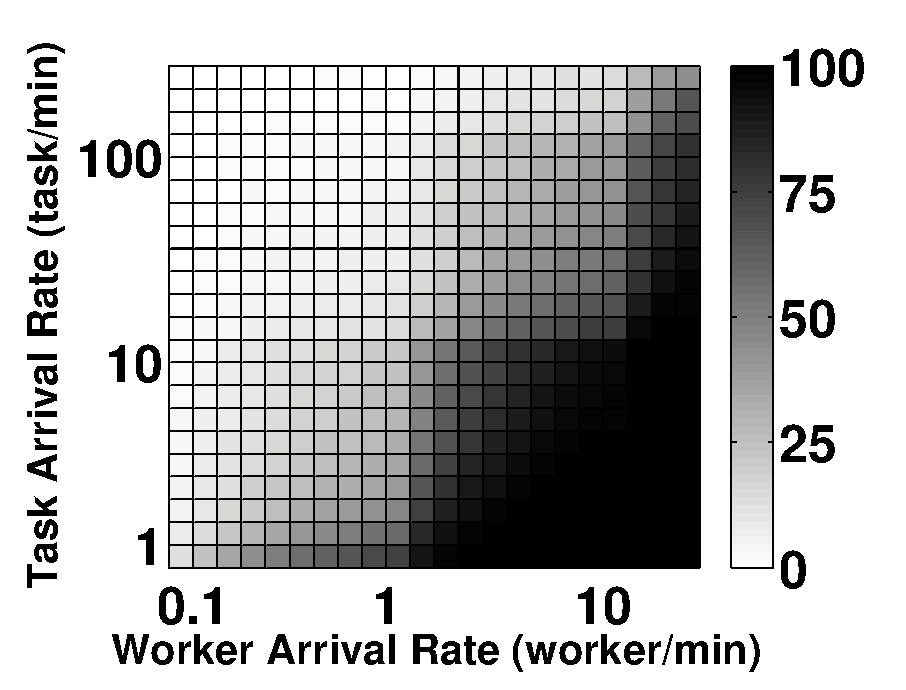
\includegraphics[width = 0.45\columnwidth]{figures/bchd.eps}
    }
    \vspace{-0.15in}
    \caption{\small{Assignment Profile-Varying Worker/Task Arrival Rates}}
    \label{fig:tw_rate}
\end{figure}

In order to study the effect of temporal parameters of SC, we ran several experiments using different pairs of task arrival rates ($t_{rate}$) and worker arrival rates ($w_{rate}$). In \cref{fig:tw_rate} we show the effect of increasing $t_{rate}$ and $w_{rate}$ on the quality of the assignment. The level of grayness corresponds to the percentage of completed tasks with black and white representing 100\% and 0\%, respectively. As we can see with small number of workers, as we increase the task arrival rate, the percentage of completed tasks decreases where at the top left corner of each plot we get close to 0\%. On the other hand in \cref{fig:nn_comp,fig:bi_comp,fig:emd_comp} for NN, BI and BD, with small number of incoming tasks, as we increase $w_{rate}$, eventually all tasks will be completed. \cref{fig:tw_rate} clearly shows that NN, BI and BD outperform Rnd, Rnk and MFT independent of the $t_{rate}$ and $w_{rate}$.

\begin{figure}[h]
	\centering
	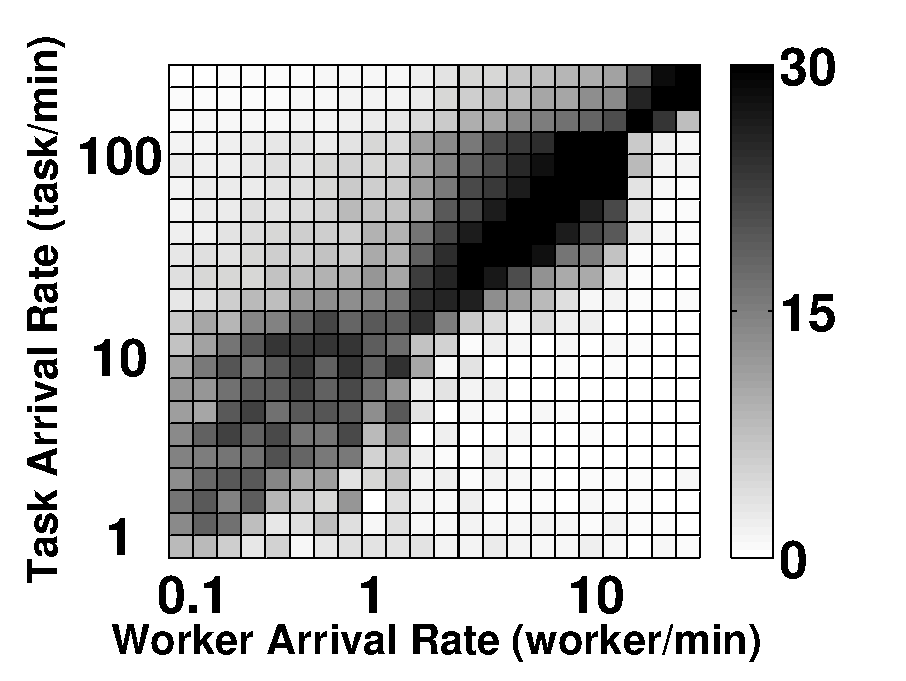
\includegraphics[width = 0.65\columnwidth]{figures/bi_nn.eps}
	\vspace{-0.1in}
	\caption{Assignment Difference of BI Vs. NN}\label{fig:bi_nn}
\end{figure}

\begin{figure}[h]
	\centering
	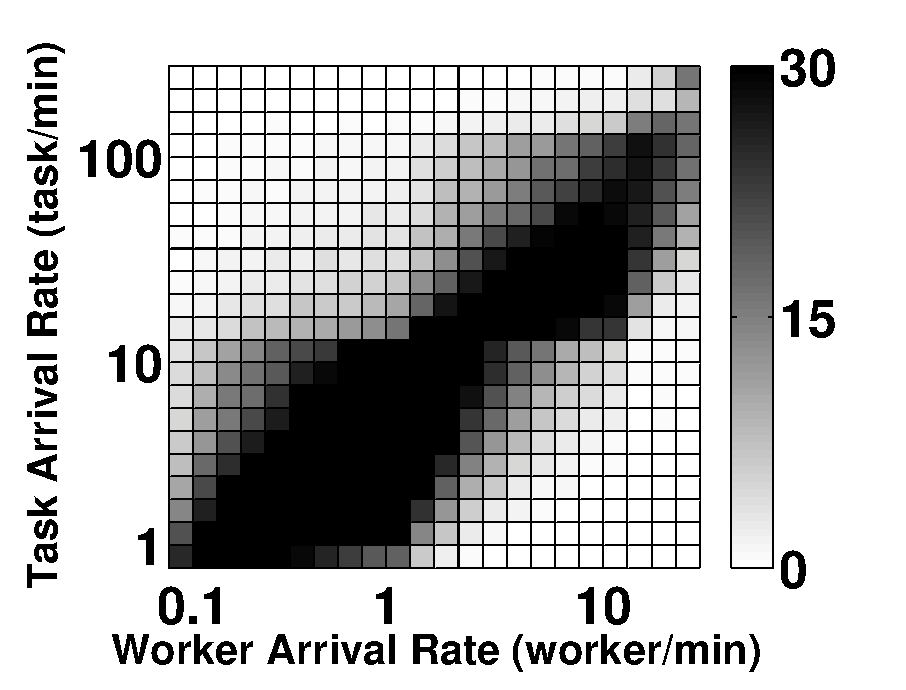
\includegraphics[width = 0.65\columnwidth]{figures/bi_bchd.eps}
	\vspace{-0.1in}
	\caption{Assignment Difference of BI Vs. BCHD}\label{fig:bi_bchd}
\end{figure}

\begin{figure}[h]
	\centering
	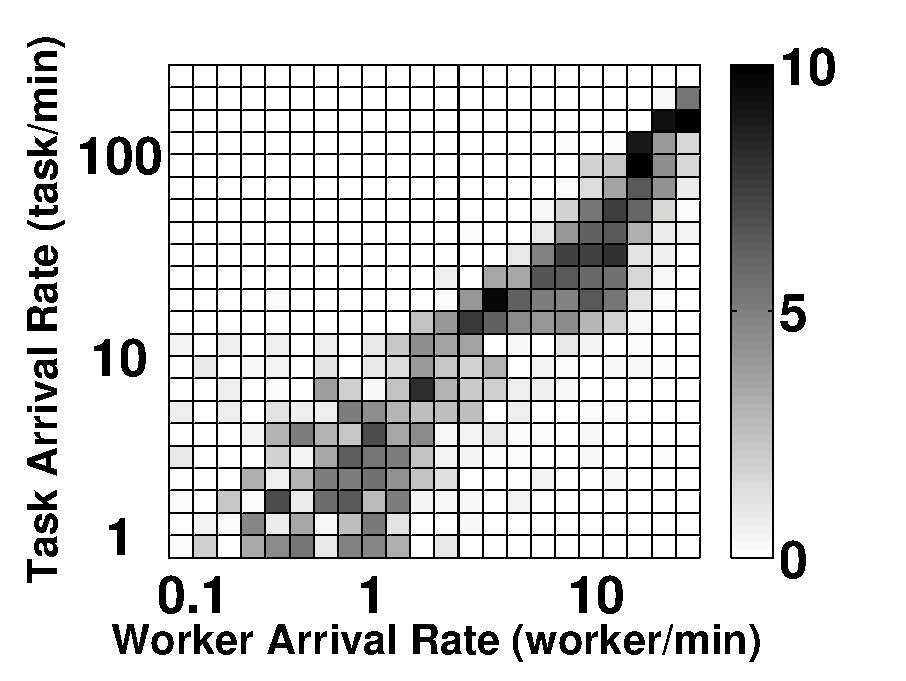
\includegraphics[width = 0.65\columnwidth]{figures/emd_bi.eps}
	\vspace{-0.1in}
	\caption{Assignment Difference of BD Vs. BI}\label{fig:emd_bi}
\end{figure}

To better evaluate the leading real-time approaches, NN, BI and BD, in \cref{fig:rate_comp} we performed a pair-wise comparison by taking their task completion rates. For example, \cref{fig:bi_nn} shows the difference between BI and NN. We observe that these three approaches perform similarly at the two extreme cases discussed in \cref{fig:tw_rate}, i.e., high task-low worker and low task-high worker. BI and BD outperform NN up to 30\% when the problem is more complex, i.e., outside the extreme cases. An interesting observation in \cref{fig:bi_nn,fig:emd_nn} is that BI and BD outperform NN by a much larger margin at scale (higher $t_{rate}$ and $w_{rate}$). The reason is that with higher higher $t_{rate}$ and $w_{rate}$ more workers are moving around and more tasks come and leave so in general the spatiotemporal dynamism of the system increases. BI and BD cope with the dynamism by guaranteeing a task gets assigned to worker that can complete it. On the contrary, NN ignores the schedule of a worker during matching and this becomes more important as there is more dynamism in the system.

\begin{figure}[h]
	\centering
	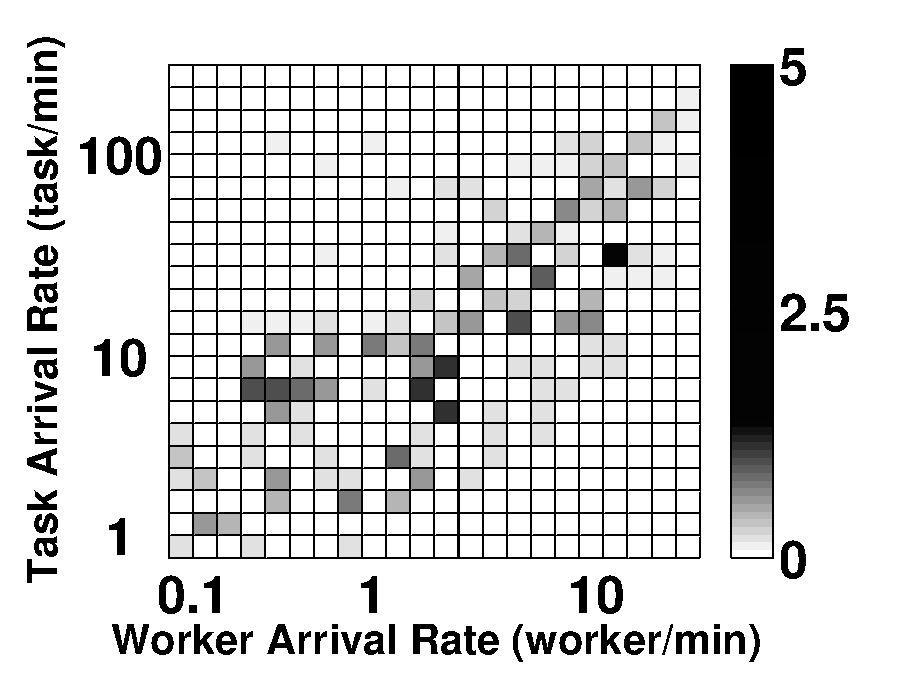
\includegraphics[width = 0.65\columnwidth]{figures/bi_abi.eps}
	\vspace{-0.1in}
	\caption{Assignment Difference of BI Vs. ApproxBI}\label{fig:bi_abi}
\end{figure}

We mentioned earlier that with the SC-rules, the workers perform an exhaustive search to find out if they can fit a new task into their schedule. As workers accept new tasks, they also complete some other tasks so as we observed in our experiments, performing an exhaustive search did not cause any scalability issues. Nevertheless, one might want to replace the exhaustive search with a polynomial time approximate algorithm. With ApproxBI, we use the insertion algorithm from \cite{Rosenkrantz74} that runs in $O(n^2)$. \cref{fig:bi_abi} shows the change affects the quality of the assignment by less than 5\%. The difference caused by ApproxBI is that the workers that are eligible for a task using BI, may not be able to fit the task in their schedules using ApproxBI due to the approximation. As a result, using ApproxBI the server may not be able to assign some tasks even if they can be completed using BI. Fortunately, as shown in \cref{fig:bi_abi}, that does not happen very often regardless of $t_{rate}$ and $w_{rate}$.

The next set of experiments compare the effect of the spatial distribution of tasks. We compared the quality of the final assignment for three different distribution. Even though real-world data usually follow a skewed spatial distribution (\cref{subsec:dataset}), the results of these experiments show that regardless of the distribution, SC rules outperform non-SC rules. With the first distribution, the location of the tasks follow a spatial Poisson process \cite{Baddeley07}. The other two distributions are a Uniform 2D distribution and a Skewed distribution. The results in \cref{fig:dists} show that SC rules generate assignments at least 20\% better than non-SC rules. Also, we can see with Poisson and Uniform distributions, there is not much difference between BI and EMD. The reason is that both distributions generate tasks at completely random locations. Consequently, tasks are released at every area with the same probability and hence EMD and BI become similar.

\begin{figure}[h]
	\centering
	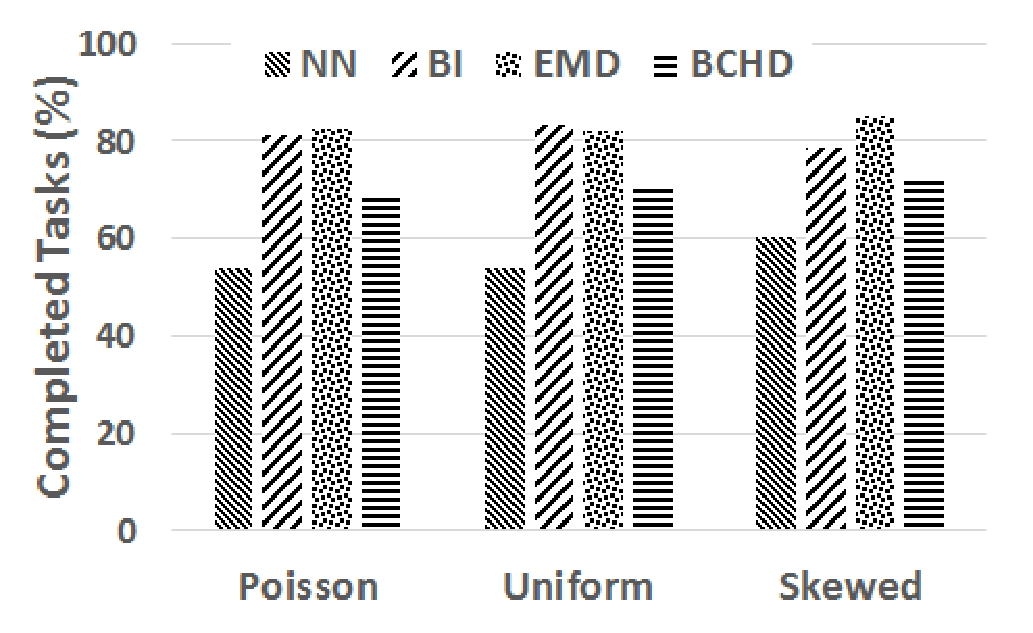
\includegraphics[width=0.75\columnwidth]{figures/dists.eps}
	\vspace{-0.1in}
	\caption{Assignment Difference-Varying Distribution}\label{fig:dists}
\end{figure}

Earlier we explained for some use cases (e.g., Uber), batched assignment does not even satisfy application requirements. Nevertheless, the results in \cref{fig:bi_lals} show even if non real-time assignments are tolerable, the quality of batched assignment is not as good as the online assignment. One reason is that the LALS algorithm performs the matching phase and then attempts to schedule tasks for their matched workers. All tasks that could not be scheduled for their matched workers, will go back to the matching phase and the process continues until all tasks are scheduled or there is no more worker to match with a task. When performing the matching, the schedule of the worker is not considered and hence a task might end up getting matched to and scheduled for a worker that was not the best worker. This in turn, can lower the chances of that worker to get assigned to a new task in the future. The second reason is that while a task is waiting at the server to get processed with the next batch, depending on the length of the batching time interval, it will lose some portion of its availability time which in turn, can lower the chances of the task fitting a worker's schedule.

\subsection{Scalability}
\label{subsec:exp_scale}
The last set of experiments focus on measuring the scalability of two system architectures, i.e., centralized and Auction-SC (decentralized). We compare the scalability of the real-time Auction-SC algorithms with the equivalent implementation of the same algorithms on a single centralized SC-Server. 

We can measure the scalability of SC systems by their throughput: the number of tasks processed per second , or equivalently, the processing time per task, shown in \cref{fig:runtime}. Because of the decentralized architecture of Auction-SC, in \cref{fig:runtime} we see that the average processing time of a single task does not change as the arrival rate of workers increases. On the contrary, with the centralized architecture, the average processing time of a single task increases linearly as we increase the number of workers and is several orders of magnitude higher than Auction-SC approaches. Although BD consumes more time than other real-time algorithms, but only takes up to 3 milliseconds.

\begin{figure}[h]
    \centering
    \subfigure[M-BI]{
        \label{fig:runtime_mbi}
        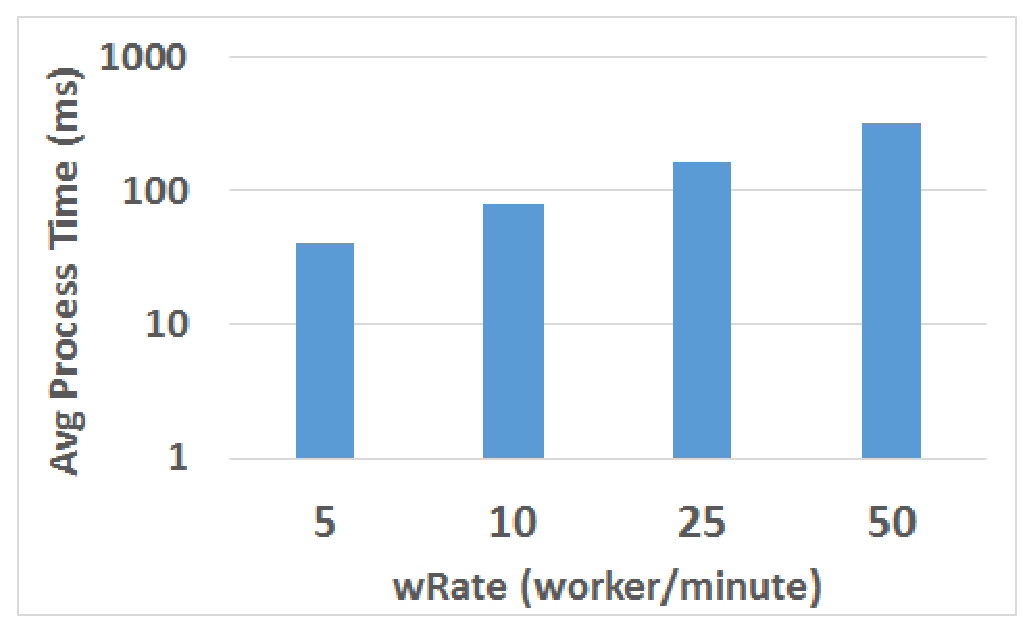
\includegraphics[width = 0.45\columnwidth]{figures/run_time_mbi.eps}
    }
    \subfigure[A-BI]{
        \label{fig:runtime_abi}
        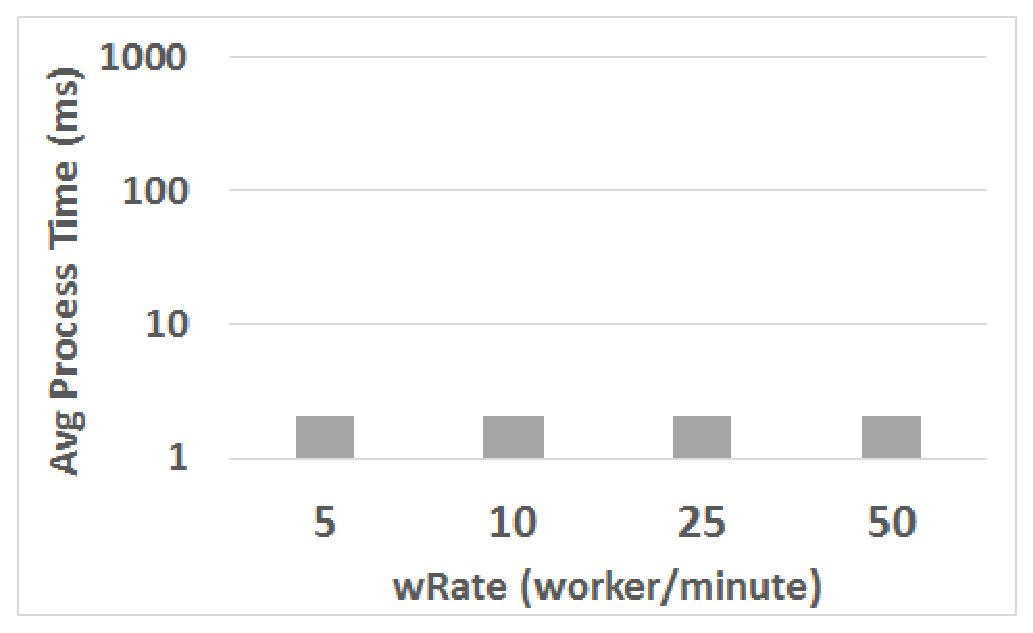
\includegraphics[width = 0.45\columnwidth]{figures/run_time_abi.eps}
    }
    \subfigure[M-BD]{
        \label{fig:runtime_mbd}
        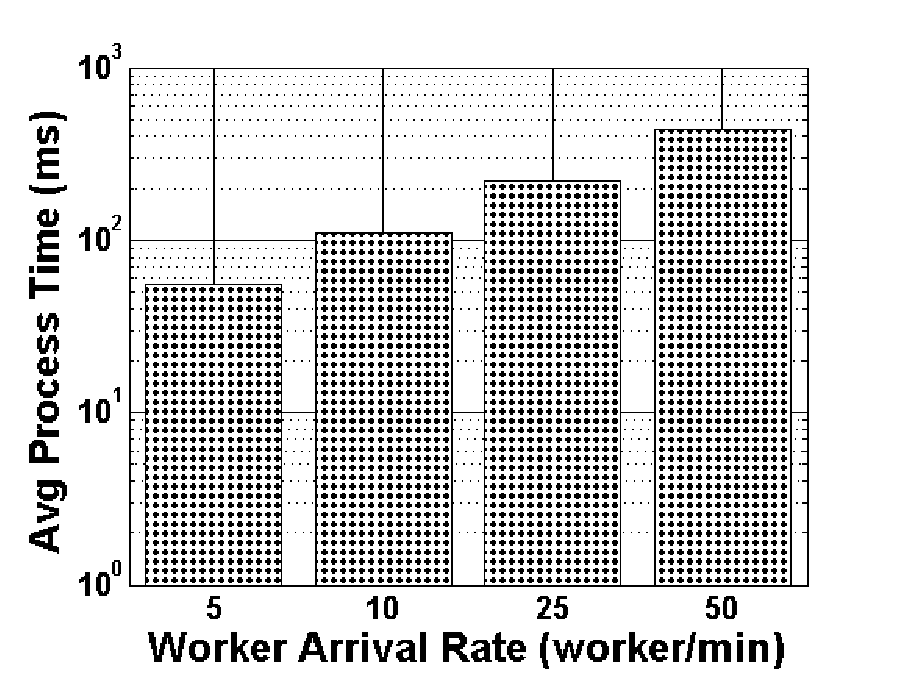
\includegraphics[width = 0.45\columnwidth]{figures/run_time_mbd.eps}
    }
    \subfigure[A-BD]{
        \label{fig:runtime_abd}
        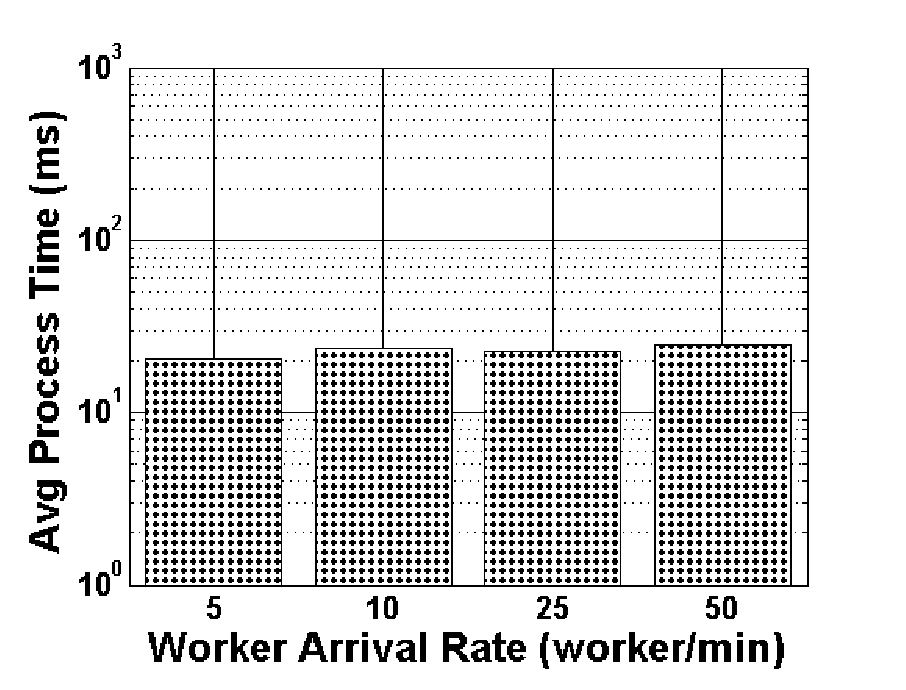
\includegraphics[width = 0.45\columnwidth]{figures/run_time_abd.eps}
    }
    \subfigure[BCHD]{
        \label{fig:runtime_bchd}
        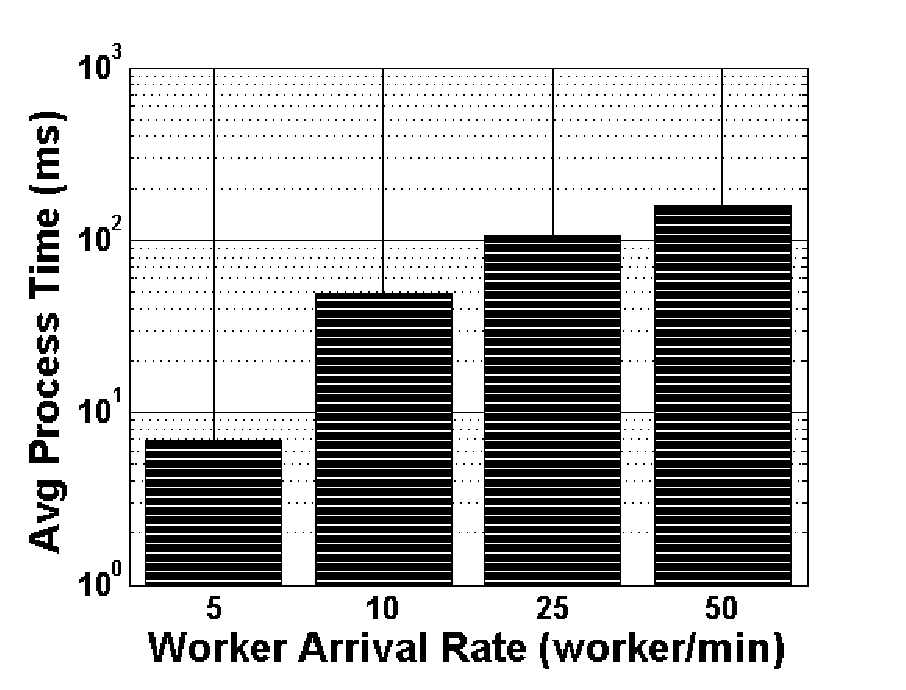
\includegraphics[width = 0.45\columnwidth]{figures/run_time_bchd.eps}
    }
    \vspace{-0.15in}
    \caption{Average processing time for a single task}
    \label{fig:runtime}
\end{figure}

For a \emph{CEP} engine, it is also common to measure the queuing delay of events \cite{Wu06} once they arrive at the system as a metric for the scalablility of the systems. In \cref{fig:queue} we compare the average queuing delay of tasks in the two architectures after running them for 1 hour. We can see that the centralized system suffers from queuing delays with less than 10 tasks/second. On the other hand, with Auction-SC, even for BD, we do not observe queuing delays for up to 500 tasks/second. To provide a more practical perspective, in \cref{fig:req} we compare the scalability of the centralized approach with Auction-SC given the current requirements of a ride sharing application in New York City \cite{NYCTaxi}, for both BI and BD bidding rules. As shown, while a centralized server is not able to satisfy the current requirements, Auction-SC can scale orders of magnitudes higher than what currently is needed. \cref{fig:queue_auc} also shows that BD incurs higher delay than BI but results in higher completion rates (\cref{fig:quality,fig:rate_comp}). Users of Auction-SC can choose between BD and BI to balance their needs for assignment quality and efficiency.

\begin{figure}[h]
	\centering
	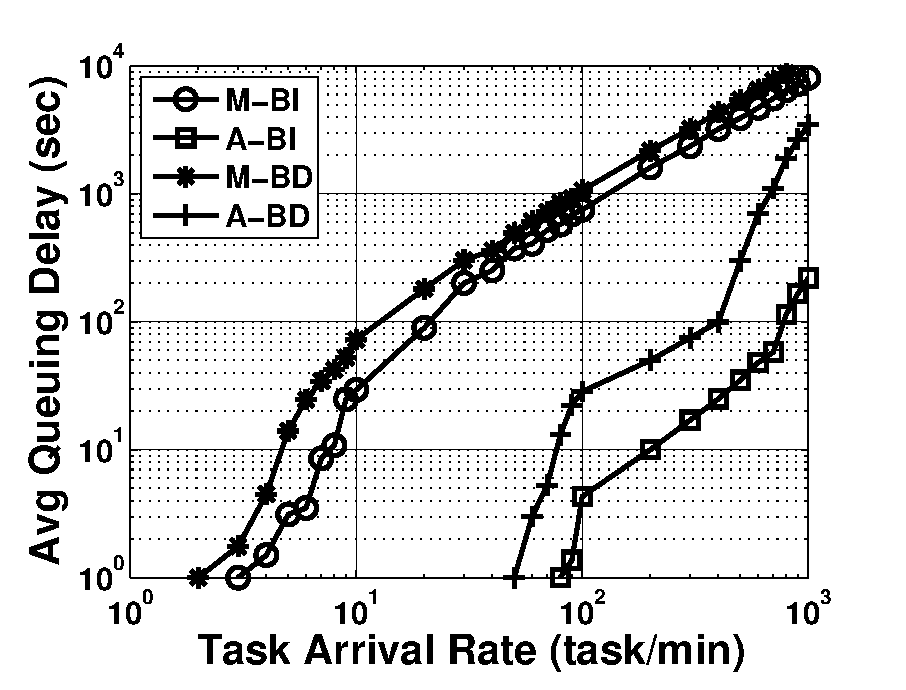
\includegraphics[width = 0.75\columnwidth]{figures/queue.eps}
	\vspace{-0.1in}
	\caption{Average queuing delay}\label{fig:queue}
\end{figure}

\begin{figure}[h]
    \centering
    \subfigure[Tasks per Batch]{
        \label{fig:bs_tpb}
        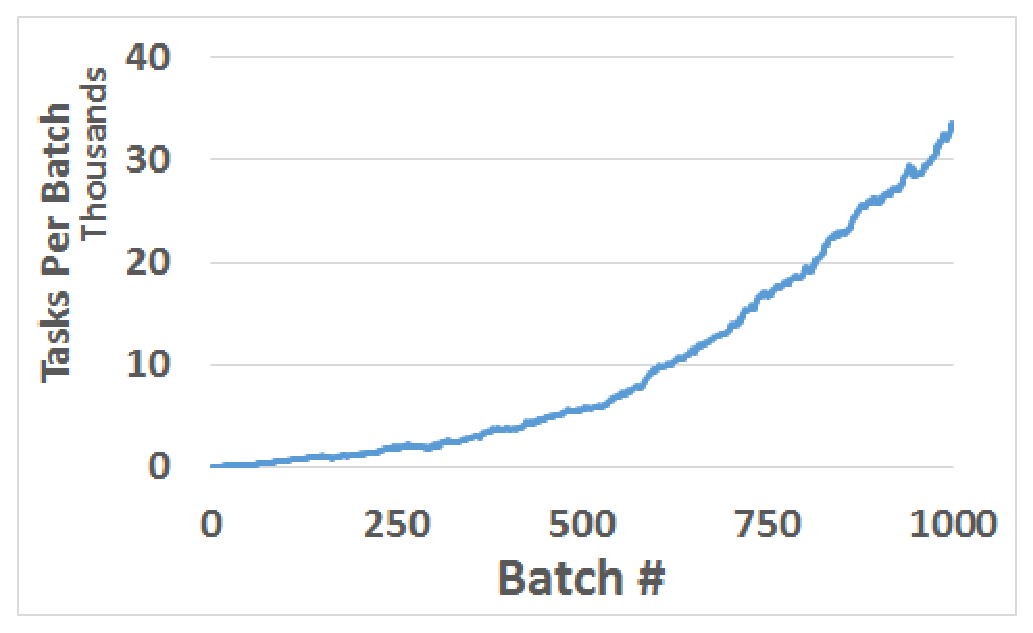
\includegraphics[width = 0.45\columnwidth]{figures/bs_tpb.eps}
    }
    \subfigure[Batch Processing Time]{
        \label{fig:bs_bpt}
        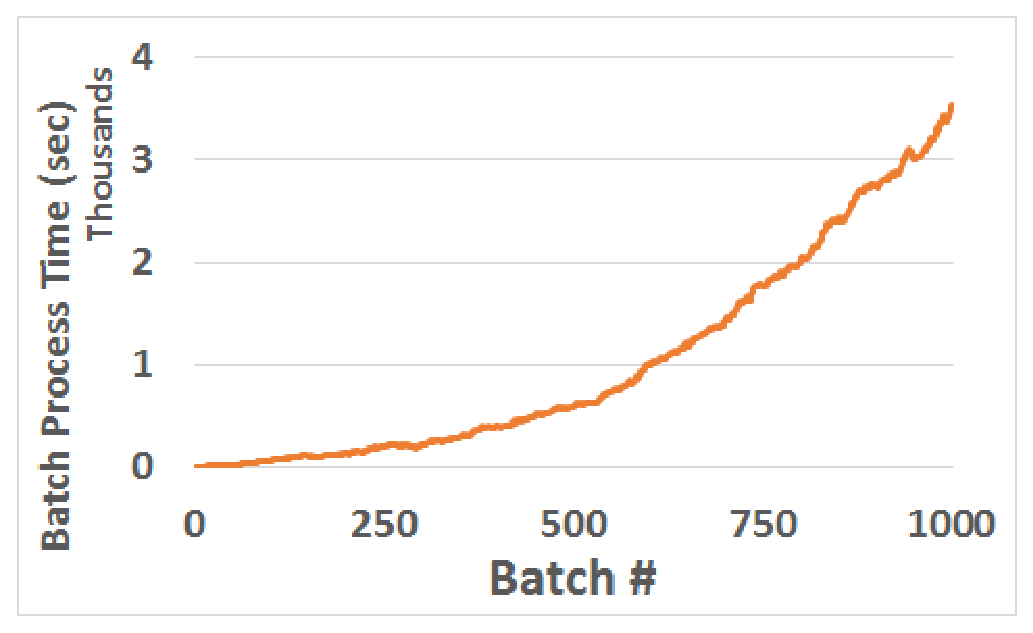
\includegraphics[width = 0.45\columnwidth]{figures/bs_bpt.eps}
    }
    \subfigure[Task Avg Delay per Batch]{
        \label{fig:bs_tad}
        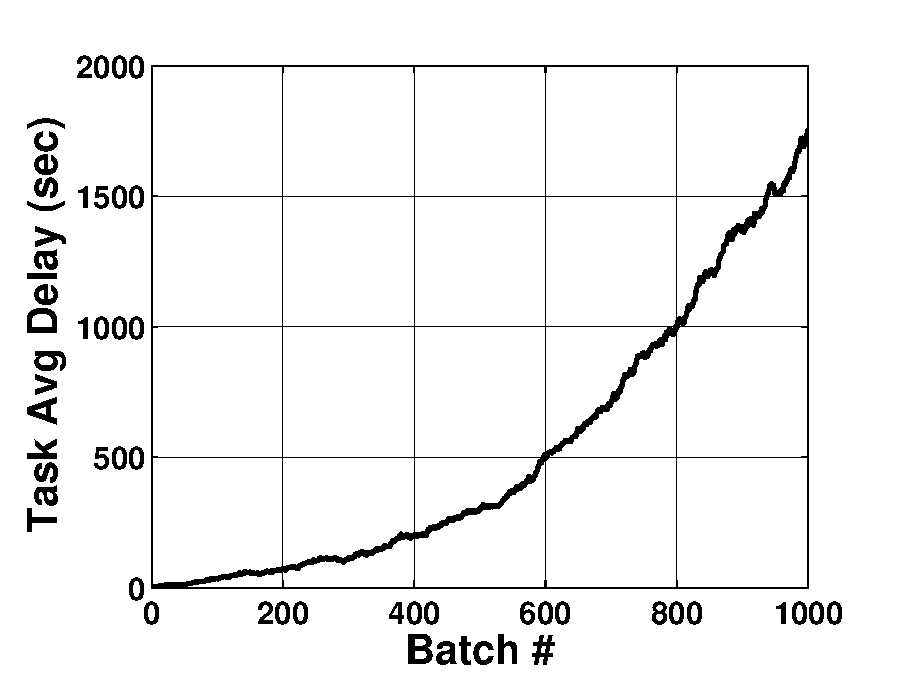
\includegraphics[width = 0.45\columnwidth]{figures/bs_tad.eps}
    }
    \vspace{-0.15in}
    \caption{BCHD Scalability ($tRate = 10 task/minute$)}
    \label{fig:runtime}
\end{figure}

\begin{figure}[h]
    \centering
    \subfigure[Tasks per Batch]{
        \label{fig:bs_tpb}
        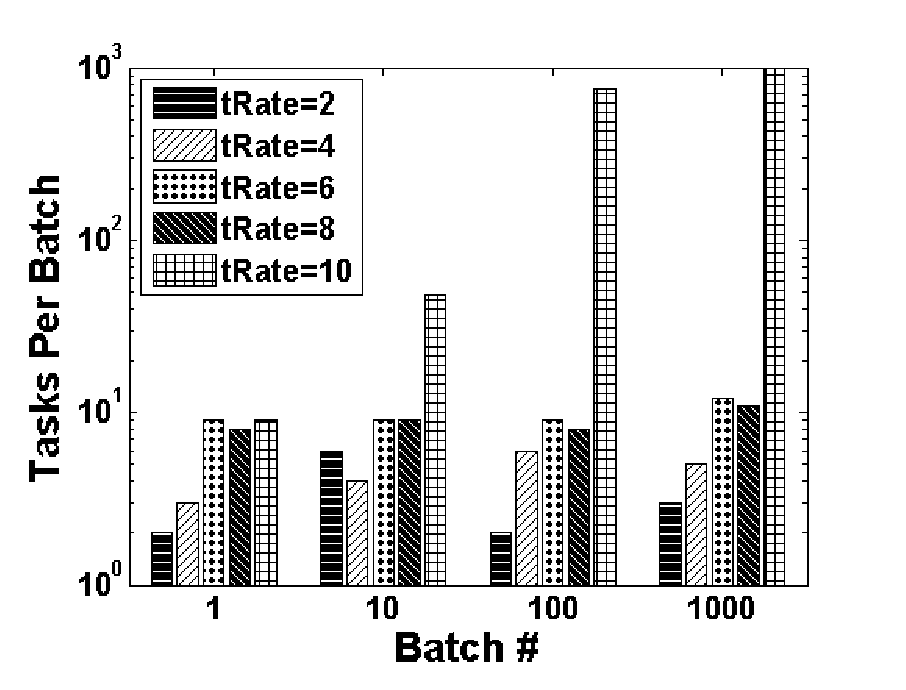
\includegraphics[width = 0.45\columnwidth]{figures/bss_tpb.eps}
    }
    \subfigure[Batch Processing Time]{
        \label{fig:bs_bpt}
        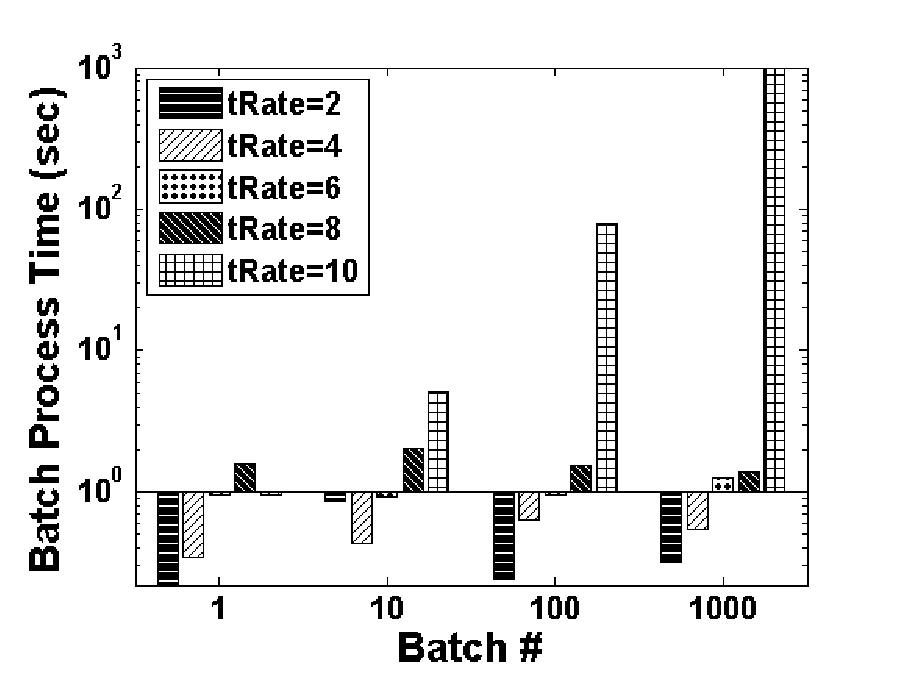
\includegraphics[width = 0.45\columnwidth]{figures/bss_bpt.eps}
    }
    \subfigure[Task Avg Delay per Batch]{
        \label{fig:bs_tad}
        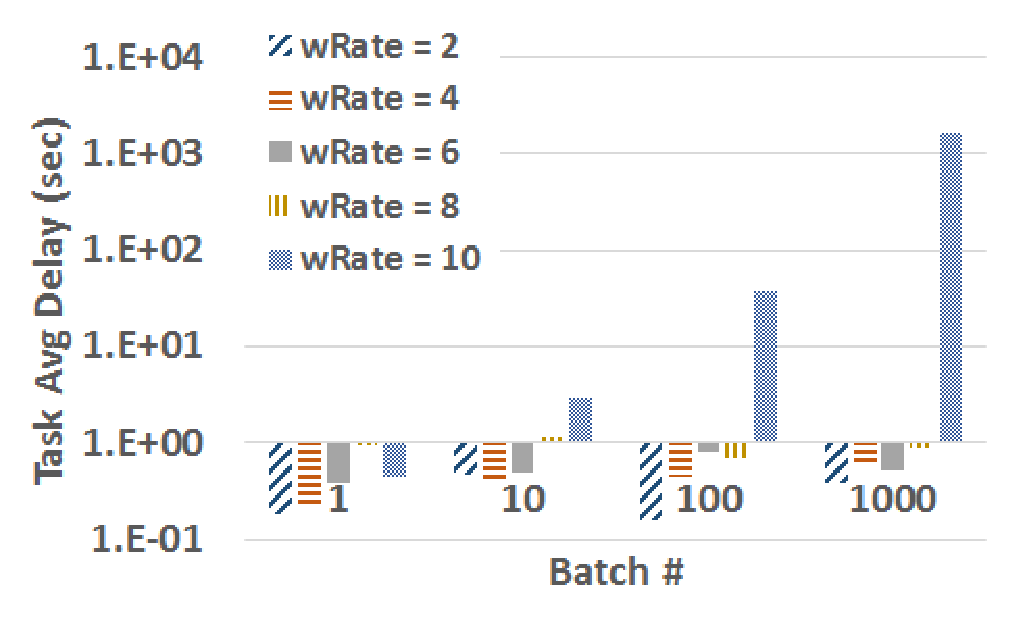
\includegraphics[width = 0.45\columnwidth]{figures/bss_tad.eps}
    }
    \vspace{-0.15in}
    \caption{BCHD Scalability}
    \label{fig:runtime}
\end{figure}

\begin{figure}[h]
	\centering
	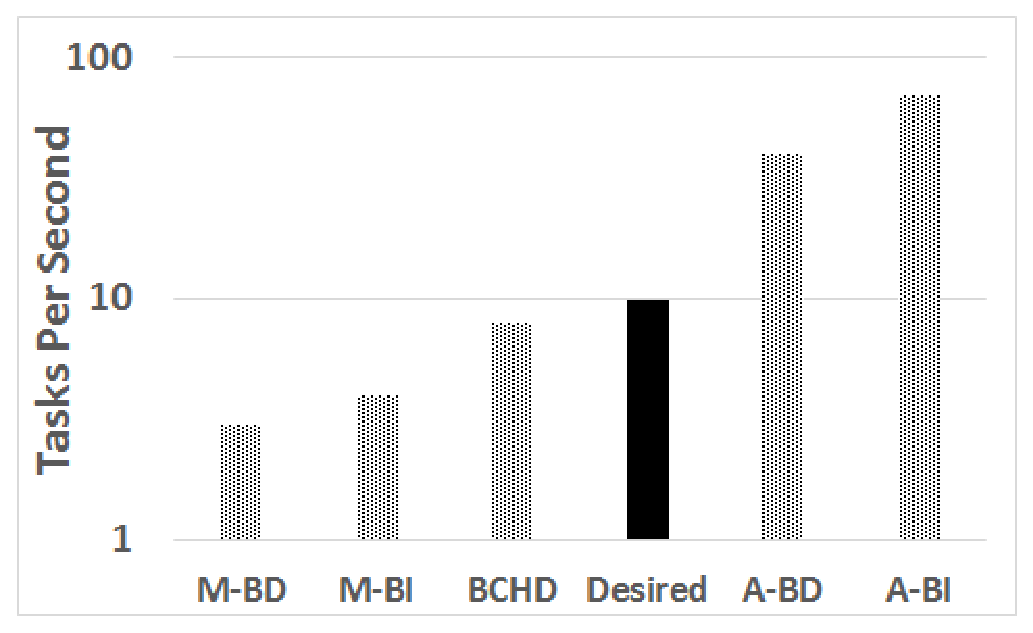
\includegraphics[width = 0.75\columnwidth]{figures/scale_req.eps}
	\vspace{-0.1in}
	\caption{Real-world Scalability Requirements}\label{fig:req}
\end{figure}

To summarize the results of our experiments, we showed that when SC bidding rules are used, the quality of the assignment is much higher as compared to when a non-SC rule is used. The consideration of scheduling at the time a task is being matched is the main reason for the better overall assignments. When running on a single centralized SC-Server, neither one of bidding rules can scale. Furthermore, the time required to process a single task increases linearly as more workers are added to the system in a centralized architecture. Scalability of a single centralized server suffers more when SC bidding rules are used due to their higher computation complexity. However, with Auction-SC we solve the scalability problem by splitting the scheduling and matching responsibilities between workers and the SC-Server. Consequently, Auction-AC can afford to execute complex SC bidding rules, resulting in a very high quality assignment. %\cref{tab:summary} shows the summary of our experimental results.

%\begin{table*}
%  \centering
%  \begin{tabular}{|c|c|c|c|c|c|c|c|c|}
%    \hline
%    \multicolumn{2}{|>{\columncolor{kugray5}}c|}{}&\multicolumn{4}{c|}{non-SC bidding rules}&\multicolumn{2}{c|}{SC bidding rules}\\
%    \arrayrulecolor{kugray5}
%    \arrayrulecolor{black}
%    \cline{3-8}
%    \multicolumn{2}{|>{\columncolor{kugray5}}c|}{}&Rnd&Rnk&NN&MFT&BI&BD\\
%    \hline
%    \multirow{2}{*}{Centralized}&Scalability&Bad&Bad&Bad&Bad&Very Bad&Very Bad\\
%    \cline{2-8}
%                         		&Assignment Quality&Very Bad&Very Bad&Bad&Very Bad&Very Good&Very Good\\
%    \hline
%    \multirow{2}{*}{Auction-SC}&Scalability&Very Good&Very Good&Very Good&Very Good&Good&Good\\
%    \cline{2-8}
%                         		&Assignment Quality&Very Bad&Very Bad&Bad&Very Bad&Very Good&Very Good\\
%    \hline
%  \end{tabular}
%  \vspace{-0.1in}
%  \caption{Summary of Experimental Results}
%  \label{tab:summary}
%\end{table*}